\chapter{The Major Key to Your Better Future Is You}

These notes follow a Jim Rohn seminar preserved in a curated LazyingArt LLC playlist, and they keep the surviving transcript as the primary source. We use the visible board frames only where they genuinely support the lecture: first as opening seminar context under the heading \emph{Personal Dev.}, and later as evidence for a narrow plus-minus comparison around the law of use. The resulting chapter keeps Rohn's spoken order: first the thesis of personal development, then the puzzle of compensation, then the seasons, responsibility, discipline and study, the basic laws, and finally goals, asking, emotional ignition, and the late warning about mental and attitudinal decay.

\section{Personal Development and the Compensation Puzzle}

Rohn opens with a thesis and its reverse. The lecture does not begin by cataloging techniques; it begins by naming a dependence relation. If we want more, we must become more. If we refuse the change in ourselves, then the visible results remain roughly where they were. This is not yet a formal economics model, but it already behaves like one: outcome depends on formation.

\begin{figure}[h]
\centering

\includegraphics[width=0.78\linewidth]{lecture_12_figure_01.png}
\caption{Opening chalkboard headed \texttt{Personal Dev.}. The frame is contextual rather than mathematical, but it anchors the seminar setting and the governing topic.}
\end{figure}

\begin{align}
\text{have more} &\Leftarrow \text{become more},\\
\neg(\text{change in self}) &\Rightarrow \text{same results}.
\end{align}

The lecture immediately sharpens this with a hard-edged heuristic about money:
\begin{equation}
\text{income} \not\!\!\gg \text{personal development}.
\end{equation}
This should be read cautiously, as Rohn means it: a lucky jump in income can happen, but unless the person grows into that new level, the money has a way of sliding back toward the level of the self that carries it.

He then adds two clarifications. First, success is attracted rather than pursued. Second, the question on the job is not only ``What am I getting?'' but also ``What am I becoming?'' In his language, happiness is not mainly contained in what one gets, but in what one becomes.

\subsection{Question \& Answer}

\paragraph{Question.} If time is the same, what makes the difference?

\paragraph{Answer.} Value.

Rohn's first real conceptual obstacle is economic. Two people may work for the same company, with the same products, in the same community, under the same traffic, the same problems, and the same apparent time budget, yet one makes twice as much as the other. His first false lead is time. He rejects it because there is no extra time to be found.

\begin{definition}
In this lecture, \emph{value} means what one brings to the marketplace beyond the mere passage of time. It is the difference-making variable in compensation.
\end{definition}

\begin{proposition}
Holding time fixed, the lecture treats compensation as tracking value brought to the marketplace rather than time alone.
\end{proposition}

\begin{proof}
Rohn asks why two people with apparently the same conditions can be paid differently. He tests time as the candidate variable and rejects it: one cannot acquire ``extra time'' beyond the common day. He then introduces value as the key word and states that value makes the difference in results. Thus the explanatory variable is shifted from time to value.
\end{proof}

A cautious worked example, faithful to the lecture's own phrasing, is the following:
\begin{align}
\text{same time} + \text{value} &\Rightarrow \text{pay},\\
\text{same time} + 2\times \text{value} &\Rightarrow \approx 2\times \text{pay},\\
\text{same time} + 3\times \text{value} &\Rightarrow \approx 3\times \text{pay}.
\end{align}
Rohn does not mean this as a precise market theorem. He means that the same clock-time can carry substantially different compensation when the person has become more valuable.

This is why the economic puzzle immediately folds back into the lecture's larger theme:
\begin{equation}
\text{success} \Leftarrow \text{work on yourself}.
\end{equation}

\section{The Major Key Is You}

After previewing the seminar's larger menu, Rohn makes the theme explicit: \emph{the major key to your better future is you}. He asks the audience to underline the words \emph{major} and \emph{you}. This is a useful clue to the lecture's logic. The point is not that external conditions are irrelevant, but that the principal term in the equation is the self.

\begin{equation}
\text{better future} \Leftarrow \text{you}.
\end{equation}

From there he recounts the clue given by Mr.\ Shoaff: for things to change for you, you have got to change. This is the pivot from motivation to law-like reasoning.

\begin{align}
\text{for things to change for you} &\Rightarrow \text{you must change},\\
\text{better life} &\Leftarrow \text{better self}.
\end{align}

The lecture then widens the frame. The tides come in and go out. It gets light and then dark. Fall is followed by winter. The point is not meteorological. The point is structural: the world is not about to reorganize itself to suit our preferences.

\subsection{Question \& Answer}

\paragraph{Question.} If life does not change, how can my life change?

\paragraph{Answer.} When we change.

The lecture states the answer in exactly that form. This is the step that prevents us from waiting for a universal easing of conditions. Once this is accepted, the next model is unavoidable: life must be read seasonally.

\section{Life as Seasons: The Four Major Lessons}

Rohn's first large model is agricultural. He does not offer a wheel or a balance sheet. He offers a sequence:
\begin{equation}
\text{winter} \to \text{spring} \to \text{summer} \to \text{fall}.
\end{equation}
What matters is not only the order, but the fact that the order is recurrent. Difficulty is not an interruption of life. Opportunity is not a permanent possession. Growth is exposed. Harvest reveals.

\begin{figure}[h]
\centering
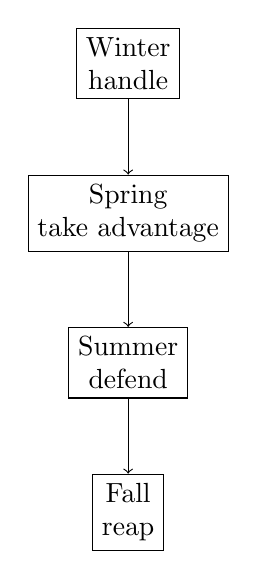
\begin{tikzpicture}[x=1cm,y=1cm]
\node[draw, align=center] (w) at (0,0) {Winter\\handle};
\node[draw, align=center] (sp) at (0,-1.9) {Spring\\take advantage};
\node[draw, align=center] (su) at (0,-3.8) {Summer\\defend};
\node[draw, align=center] (f) at (0,-5.7) {Fall\\reap};
\draw[->] (w.south) -- (sp.north);
\draw[->] (sp.south) -- (su.north);
\draw[->] (su.south) -- (f.north);
\end{tikzpicture}
\caption{Transcript-derived seasonal model, kept narrow and vertical for pocket-size layout.}
\end{figure}

The lecture compresses the four lessons into a memorable sequence:
\begin{align}
\text{winter} &\Rightarrow \text{handle},\\
\text{spring} &\Rightarrow \text{take advantage},\\
\text{summer} &\Rightarrow \text{defend},\\
\text{fall} &\Rightarrow \text{reap without complaint}.
\end{align}

Winter names difficulty: recessions, smashed plans, broken hearts, confusion, disappointment. The lecture does not promise the removal of winter. It asks for a different response to it. January cannot be torn off the calendar. But one can get stronger, wiser, and better. Hence the lecture's practical restatement:
\begin{equation}
\text{you cannot change the seasons} \Rightarrow \text{you can change yourself}.
\end{equation}

Spring is opportunity. The difficulty here is not waiting for opportunity to appear; it is using it once it comes. Spring must be taken advantage of quickly. One of Rohn's hardest lines belongs here: in life one must get good either at planting in the spring or begging in the fall.

Summer is the season of defense. Good beginnings are not left alone. Gardens are invaded; values are attacked. The lecture insists that every value must be defended: political, social, family, business, and personal.

Fall is harvest. It is also the season in which responsibility is hardest to evade. We are asked to reap without apology if we have done well, and without complaint if we have not.

\section{Responsibility, Blame, and the Difference-Making Variable}

The movement from seasons to responsibility is exact. If winter and spring are common conditions, then the decisive question is no longer what has happened, but what we have done with it. Rohn builds this with a long blame-list: government, taxes, prices, weather, traffic, car, company, training program, relatives, neighbors, economy, community. The list matters because it prepares the turning sentence.

Mr.\ Shoaff's blunt correction is simple: \emph{You ain't on it}. The self is missing from the explanation.

\subsection{Question \& Answer}

\paragraph{Question.} What actually determines the quality of life once happenings are shared?

\paragraph{Answer.} Our response. In Rohn's repeated formula: what you do.

\begin{proposition}
If many external happenings are common, then the difference-making term is response rather than event.
\end{proposition}

\begin{proof}
Rohn argues that the sun went down on all of us last night, and that the same storm can confront two salesmen in the same morning. One stays home and one goes out because the empty roads improve the day for selling. Since the event is common and the outcome differs, the decisive variable is response.
\end{proof}

The maxim should therefore be preserved in displayed form:
\begin{align}
\text{life quality} &\not\Leftarrow \text{what happens},\\
\text{life quality} &\Leftarrow \text{what you do}.
\end{align}

We can write the rainstorm example schematically:
\begin{align}
\text{same storm} + \text{withdraw} &\Rightarrow \text{one result},\\
\text{same storm} + \text{act} &\Rightarrow \text{another result}.
\end{align}
Again, this is not a formal probabilistic model. It is a disciplined piece of practical reasoning.

This section ends with one of the lecture's strongest forward transitions: starting tomorrow, what will we do that changes the direction of our lives? Once that question is asked, inspiration alone is no longer enough. We need mechanism.

\section{Discipline, Study, and Learning the Setup}

Rohn now turns from declaration to process. He insists that life change takes more than philosophical pronouncement, and more than enthusiasm. One may arrive at the gym highly enthusiastic about lifting two hundred pounds, but a second term is required there. That term is discipline.

\begin{definition}
\emph{Discipline}, in this lecture, is the capacity to make oneself do the necessary thing, beginning with small acts and letting them build the muscle required for larger ones.
\end{definition}

The key move here is scalar. One begins with the small disciplines. Little acts are not trivial; they are the training ground for larger acts. Rohn's logic is cumulative: little disciplines lead to big ones, and without them the big challenges cannot be handled.

He adds self-motivation. This is not a decorative phrase. It means that change cannot be outsourced. We may train people, encourage them, or recruit them, but each person must finally change himself.

From there the lecture takes one more step inward:
\begin{equation}
\text{idea} \to \text{journal} \to \text{repetition} \to \text{action}.
\end{equation}
Ideas matter because they alter the possibilities one can even see. The journal matters because the mind is not meant to be a filing cabinet. Repetition matters because an idea must be revisited until it takes root in conduct.

This is where Rohn introduces \emph{study}. If one wishes to be successful, study success; if happy, study happiness; if wealthy, study wealth. The thought is not mystical. It is operational. Study is the disciplined acquisition of the forms of life one hopes to inhabit.

He then expands study into a broader notion: the \emph{setup}.

\begin{definition}
The \emph{setup} is Rohn's name for the law-governed arrangement of life on this planet. We did not create it, but we are placed inside it and must learn it.
\end{definition}

The lecture gives two reasons for learning the setup:
\begin{align}
\text{learn} &\Rightarrow \text{avoid harm},\\
\text{learn} &\Rightarrow \text{benefit}.
\end{align}

The first reason is defensive. Ignorance hurts. The second is positive. The same world that contains tragedy also contains happiness, prosperity, and good feeling. The task is to get on the good side of the way things work. This defensive-positive split will reappear in the next section as a visible minus-plus layout.

\section{Basic Laws: Use and Sowing}

At this point the lecture becomes most equation-like. It does so without abandoning ordinary language. The first law is the law of use.

\begin{figure}[h]
\centering

\includegraphics[width=0.72\linewidth]{lecture_12_figure_03.png}
\caption{Plus-minus comparison on the board during the law of use. The visible structure is secure; the exact chalk wording is not.}
\end{figure}

The board image gives us a visible comparison layout: a minus sign on the left, a plus sign on the right, and a partial underlined word ending in \texttt{use}. We should not pretend the full board sentence is legible. But the transcript supplies the law clearly:
\begin{equation}
\text{whatever you do not use} \Rightarrow \text{you lose}.
\end{equation}

\begin{remark}
The nearby cleaned comparison is transcript-led, not a literal transcription of the obscured chalkboard.
\end{remark}

\begin{figure}[h]
\centering
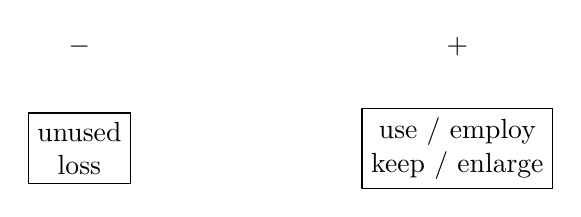
\begin{tikzpicture}[x=1cm,y=1cm]
\node at (-2.4,0.9) {$-$};
\node[draw, align=center] at (-2.4,-0.4) {unused\\loss};
\node at (2.4,0.9) {$+$};
\node[draw, align=center] at (2.4,-0.4) {use / employ\\keep / enlarge};
\end{tikzpicture}
\caption{A cautious reconstruction of the visible plus-minus comparison. The positive side is interpretive and should be read as a transcript-based summary.}
\end{figure}

Rohn derives the law concretely. Tie the arm to the body and leave it unused long enough, and the arm loses function. Then generalize:
\begin{align}
\text{faith unused} &\Rightarrow \text{decrease},\\
\text{energy unused} &\Rightarrow \text{decrease},\\
\text{talent unused} &\Rightarrow \text{loss},\\
\text{ability unused} &\Rightarrow \text{loss}.
\end{align}

A worked derivation, in the lecture's own spirit, is:
\begin{enumerate}
\item Prevent a capacity from being exercised.
\item Leave that condition in place long enough.
\item Observe decay or forfeiture of the capacity.
\item Extend the same logic from bodily use to ambition, faith, vitality, courage, and ability.
\end{enumerate}
The conclusion is practical rather than abstract: take a new inventory of yourself and make sure what is present is being used.

\subsection{Question \& Answer}

\paragraph{Question.} What do we do with a law or arrangement we may not like?

\paragraph{Answer.} Learn it anyway: first so that we do not get hurt, and second so that we can benefit.

The lecture then moves to the law of sowing and reaping. First it is given in the familiar direction:
\begin{equation}
\text{whatever you sow} \Rightarrow \text{you reap}.
\end{equation}
Then it is reversed to locate causality more sharply:
\begin{equation}
\text{whatever you reap} \Rightarrow \text{what you have sown}.
\end{equation}
That reversal matters. It takes us from complaint about the harvest to inspection of the planting.

The surviving transcript securely supports the following spine of the numbered discussion:
\begin{enumerate}
\item If you sow bad, you reap bad.
\item If you sow good, you reap good.
\item You reap more than what you sow.
\item Sometimes you lose anyway.
\item If you do not sow, you do not reap.
\end{enumerate}

The third point is the most mathematically interesting:
\begin{equation}
\text{sowing} \Rightarrow \text{more than was sown}.
\end{equation}
This is true on both sides. The lecture's negative example is:
\begin{equation}
\text{sow to the wind} \Rightarrow \text{reap the whirlwind}.
\end{equation}

The sixth point in the lecture's full numbering is the hard qualification: one may still lose. The farmer may sow well, labor honorably, and see the crop destroyed by hail the day before harvest. That is not treated as a refutation of the law. It is treated as part of the arrangement of the planet. The law is not replaced by fairness; it operates inside a world where contingency remains.

\section{Goals, Reasons, Asking, and the Day of Change}

After the break, the lecture resets into goal setting. The reset is pedagogically important. Once laws are in place, one must decide what to do within them. Rohn's first principle here is that reasons come before answers:
\begin{equation}
\text{reasons} \to \text{answers}.
\end{equation}
This is not sentiment. It is a claim about activation. One may have enough intelligence and ability and yet remain inert because the motive structure is too weak.

He then divides goals into two large classes:
\begin{equation}
\text{goals} = \text{long range} + \text{short range}.
\end{equation}
Long-range goals are dreams. Short-range goals are confidence builders for tomorrow, this week, this month, and this year.

\begin{figure}[h]
\centering
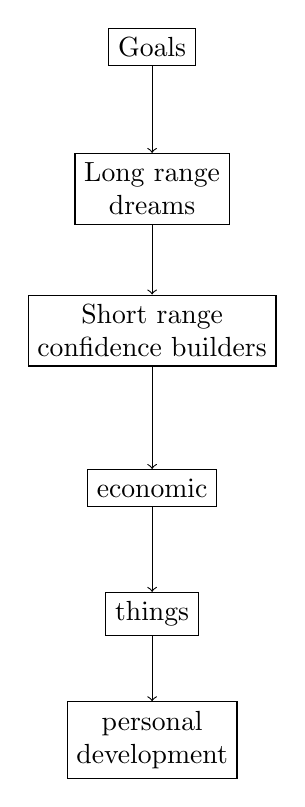
\begin{tikzpicture}[x=1cm,y=1cm]
\node[draw, align=center] (g) at (0,0) {Goals};
\node[draw, align=center] (lr) at (0,-1.8) {Long range\\dreams};
\node[draw, align=center] (sr) at (0,-3.6) {Short range\\confidence builders};
\node[draw, align=center] (e) at (0,-5.6) {economic};
\node[draw, align=center] (t) at (0,-7.2) {things};
\node[draw, align=center] (p) at (0,-8.8) {personal\\development};
\draw[->] (g.south) -- (lr.north);
\draw[->] (lr.south) -- (sr.north);
\draw[->] (sr.south) -- (e.north);
\draw[->] (e.south) -- (t.north);
\draw[->] (t.south) -- (p.north);
\end{tikzpicture}
\caption{Goal taxonomy compressed into a narrow vertical stack for pocket-size readability.}
\end{figure}

Within short-range goals he identifies three categories:
\begin{equation}
\text{short range goals} \supset \{\text{economic},\ \text{things},\ \text{personal development}\}.
\end{equation}

The lecture is especially sharp about planning:
\begin{equation}
\text{future improves by plan, not by hope}.
\end{equation}
Hope is not denied, but passive hope is treated as an affliction. One works on goals, writes them down, and checks their size and kind because goals are not inert descriptions. They affect the person carrying them. They affect the handshake, attitude, personality, walk, talk, and dress.

\subsection{Question \& Answer}

\paragraph{Question.} Is receiving the problem?

\paragraph{Answer.} No. Failure to ask is the problem.

The lecture's asking law is direct:
\begin{align}
\text{ask} &\Rightarrow \text{receive},\\
\text{asking} &\Rightarrow \text{beginning of receiving},\\
\neg(\text{ask}) &\Rightarrow \text{failure to receive}.
\end{align}

The point is then strengthened by analogy. Receiving is like the ocean: there is plenty. The problem is not that the ocean is empty; the problem is that some people go to it with a teaspoon. Asking, then, must be done in two ways. One asks with intelligence, meaning specificity, and one asks with faith, meaning a childlike capacity to believe what has been properly planned.

Rohn's compact formula for the emotional side of life change can be preserved as:
\begin{equation}
\text{disgust} \to \text{decision} \to \text{desire} \to \text{resolve} \to \text{action}.
\end{equation}
Disgust says, ``I have had it.'' Decision cuts the inner civil war. Desire is triggered from within, often by events that awaken it. Resolve says, ``I will,'' and action converts all of the preceding states into results.

The lecture then returns, surprisingly but correctly, to the diseases of attitude. This is not a digression. It is the negative half of the same machinery. Overcaution refuses risk. Pessimism feeds on faults and sees difficulty first. Poor thinking habits poison the mental factory. Complaining can cancel the future.

\begin{definition}
Rohn's \emph{mental factory} is the mind understood as a place into which thoughts pour ingredients and from which the economic, social, and personal fabric of life is built.
\end{definition}

Hence the lecture's compact mental law:
\begin{equation}
\text{as you think} \Rightarrow \text{so you become}.
\end{equation}

The sugar-strychnine example belongs here. Life contains both good and poison. It matters what is dropped into the coffee, and it matters because the mind processes it into conduct. This leads to one of the lecture's strongest late warnings: stand guard at the door of the mind. The right ingredients build; the wrong ones corrode. Complaining is not merely wasted sound. It is a destructive feed into the system.

\section{Summary}

The chapter's structure is simple even when the lecture is expansive. We begin with the relation between becoming and having. We pass from compensation to value, from value to self-change, and from self-change to the seasons. The seasons teach handling, using, defending, and reaping. Responsibility then identifies the crucial variable: not what happens, but what we do. Discipline, study, and learning the setup prepare us for the basic laws. The law of use and the law of sowing and reaping formalize consequence. Goals, reasons, and asking supply direction and activation. Finally, the emotional chain drives action, while overcaution, pessimism, polluted thought, and complaint threaten to undo the whole enterprise. The major key to the better future is therefore not an external rearrangement of the world, but the organized development and disciplined use of the self.